\documentclass{article}

\usepackage[margin=1in]{geometry}
\usepackage{color}
\usepackage{hyperref}
\usepackage{soul}
\usepackage{float}
\usepackage{amsmath}
\usepackage{framed}
\usepackage[sc]{mathpazo}
\linespread{1.20}
\usepackage[T1]{fontenc}
\usepackage{microtype}
\usepackage{listings}
\usepackage{graphicx}
\usepackage{courier}
\usepackage{enumitem}
\usepackage{lipsum}
\usepackage{verbatim}

\definecolor{mygreen}{rgb}{0,0.6,0}
\definecolor{light-gray}{gray}{0.95}

\lstset{basicstyle=\footnotesize\ttfamily,breaklines=true,language=Matlab}
\lstset{frame=single,commentstyle=\color{mygreen}}
\lstset{aboveskip=0.5cm,belowskip=0.3cm}
\lstset{backgroundcolor=\color{light-gray}}

\graphicspath{ {./images/} }

\hypersetup{pdfpagemode=UseNone}

\newcommand{\todo}[1] {\hl{TODO: #1}}

\setlength{\parindent}{0cm}

\begin{document}

\title{The Classification of Individual Digits \\ using Pattern Recognition Techniques}
\author{Tom Runia \& Arnold Schutter}

\maketitle

Optical Character Recognition (OCR) is the conversion of scanned images containing written or printed text into machine-encoded text using pattern recognition. It is widely used in our modern world, for example to automatically read out passport documents or bank statements. In this paper we employ various pattern recognition techniques to classify individual digits in bank account numbers. The implementation is done using Matlab and the pattern recognition toolbox PRtools \cite{prtools-manual}. This article was written as part of the graduate course Pattern Recognition given at Delft University of Technology.

\section{Introduction}
The goal of this paper is to research the possibilies of using pattern recognition techniques to classify individual handwritten digits on bank statements. There are two scenarios that we are interested in. In the first scenario the OCR system is only trained once and then applied to the field. The second scenario allows the system to be trained for each batch of cheques. Both of these scenarios are worked out by training and testing on the standard dataset of handwritten digits which is available for free through the US National Institute of Standards \& Technologies (NIST). \\

The strucure of this article is as follows. We start off by discussing the first scenario and presenting our solution to the problem. Also we report our design choices and present some test results regarding the classification performance. Then we continue by discussing the second scenario in the same manner. Finally we review our work in the conclusion and give some recommendations for future work.

\section{Scenario 1: \textit{System is trained once}}

As already mentioned, this scenario only allows the recognition system to be trained once. After this initial training phase the system should be able to recognize individual digits with an error rate lower than $5\%$. This means that we should use a large amount of training data in order to allow accurate classification. Because of the presence of a lot of training data, there are many ways to train a classifier. We will try to find an optimum between the amount of features, the kind of features, the manipulation of them and the classifier. 

\subsection{Classification on Raw Pixel Data}
The first way of classifying is to use the raw pixels of the image without filtering or adding extra features. Since the images contain $256 \times 256$ pixels, using all the pixels yields an amount of features bigger than the size of the training set. To avoid the \emph{curse of dimensionality} we lower the amount of features by scaling the images with the image-mapping tools in \texttt{PRTools}. The optimal size and the optimal way of interpolating the pixels is found empirically. For the classification are complex classifiers preferred above less complex classifiers, since the high number of available features. However, to make it possible to compare different classifiers on different pixel-sizes, also less complex classifiers are used such as \textit{linear discriminant classifier} and \textit{nearest-mean classifier}. The results of using various classifiers are shown in Table~\ref{table:results-only-pixels}.

% Table of classifiers on raw pixels
\begin{table}[H]
  \small
  \centering
    \begin{tabular}{l|l|llllll|}
    \hline
    Interpolation & Pixels & Parzen & ldc   & qdc   & Fisher & nmc & knnc \\
		\hline
    \textbf{Bicubic} & 8x8   & \textbf{0,039} & 0,109 & 0,054 & 0,136 & 0,189 & 0,046 \\
    \textbf{} & 9x9   & \textbf{0,036} & 0,67  & 0,191 & 0,129 & 0,193 & 0,049 \\
    \textbf{} & 10x10 & \textbf{0,021} & 0,885 & 0,488 & 0,12  & 0,15  & 0,023 \\
    \textbf{} & 11x11 & \textbf{0,03} & 0,899 & 0,65  & 0,141 & 0,187 & 0,032 \\
    \textbf{} & 12x12 & \textbf{0,044} & 0,897 & 0,675 & 0,159 & 0,194 & \textbf{0,044} \\
    \textbf{} & 13x13 & \textbf{0,041} & 0,9   & 0,69  & 0,146 & 0,198 & 0,042 \\
		\hline
    \textbf{Nearest} & 8x8   & \textbf{0,109} & 0,16  & 0,352 & 0,177 & 0,213 & 0,13 \\
    \textbf{} & 9x9   & \textbf{0,114} & 0,164 & 0,325 & 0,186 & 0,221 & 0,131 \\
    \textbf{} & 10x10 & \textbf{0,108} & 0,833 & 0,532 & 0,165 & 0,208 & 0,11 \\
    \textbf{} & 11x11 & \textbf{0,085} & 0,887 & 0,711 & 0,171 & 0,217 & 0,103 \\
    \textbf{} & 12x12 & \textbf{0,083} & 0,9   & 0,763 & 0,146 & 0,191 & 0,088 \\
    \textbf{} & 13x13 & \textbf{0,096} & 0,898 & 0,784 & 0,169 & 0,222 & 0,107 \\
		\hline
    \textbf{Bilinear} & 8x8   & \textbf{0,029} & 0,111 & 0,049 & 0,14  & 0,188 & 0,032 \\
    \textbf{} & 9x9   & \textbf{0,047} & 0,798 & 0,284 & 0,142 & 0,203 & 0,049 \\
    \textbf{} & 10x10 & \textbf{0,032} & 0,895 & 0,579 & 0,14  & 0,199 & 0,038 \\
    \textbf{} & 11x11 & \textbf{0,039} & 0,898 & 0,689 & 0,151 & 0,192 & 0,042 \\
    \textbf{} & 12x12 & 0,041 & 0,899 & 0,719 & 0,147 & 0,198 & \textbf{0,04} \\
    \textbf{} & 13x13 & \textbf{0,04} & 0,9   & 0,712 & 0,134 & 0,16  & \textbf{0,04} \\
		\hline
    \textbf{} & Best  & \textbf{0,021} & 0,109 & 0,049 & 0,12  & 0,15  & 0,023 \\
    \hline
    \end{tabular}%
		\caption{Error rates of various classifiers using pixels with different sizes and scaling types 
		\label{table:results-only-pixels}}
\end{table}

The results in the table show that the \emph{Parzen} and \emph{k-nearest neighbor} classifiers perform best, the latter performs above expectations. The good performance of the k-nearest neighbor classifier raises the idea that the pixels per class cluster well. The \emph{quadratic bayes normal classifier} (qdc) performs a bit worse, from this we conclude that the measurements of each class are not well normally distributed. As expected, the rest of the classifiers which are less complex perform worse. \\

Another classifier that we use is the \textit{support vector classifier (svc)}, which is a more complex classifier. This classifier is mentioned seperately, because its performance depends on a lot of parameters. The classifier is able to use different kernels which are listed below and also it can vary the weights used for the features.

\begin{itemize}[noitemsep]
    \item Polynomial kernel (P)
    \item Exponential kernel (E)
    \item Radial kernel (R)
    \item Sigmoid kernel (S)
    \item Distance kernel (D)
    \item Minkowski kernel (M)
    \item City-Block kernel (C)
\end{itemize}

We noticed that only for the \emph{polynomial} and \textit{radial} kernels it was really useful to change the weight. Therefore the error-rates for the classifications with optimal weights for these kernels are shown in the tabel. Some of the kernels are ignored, since their results were not good enough. The error-rates for different images sizes and interpolation methods are shown in Table~\ref{table: error rate SVC} . 

% Table generated by Excel2LaTeX from sheet 'Sheet1'
\begin{table}[H]
  \small
  \centering
    \begin{tabular}{l|l|ccccccc|}
    \hline
    Interpolation & Pixelsize & P     & P ($w=2$) & S     & D     & R     & R ($w=2,5$) & E \\ 
    \hline
    \textbf{Bicubic} & 8x8   & 0,045 & 0,035 & 0,668 & 0,172 & 0,05  & \textbf{0,029} & 0,033 \\
    \textbf{} & 9x9   & 0,045 & 0,031 & 0,666 & 0,188 & 0,111 & \textbf{0,025} & 0,034 \\
    \textbf{} & 10x10 & 0,048 & 0,028 & 0,73  & 0,187 & 0,222 & \textbf{0,024} & 0,031 \\
    \textbf{} & 11x11 & 0,046 & \textbf{0,024} & 0,769 & 0,177 & 0,319 & 0,026 & 0,05 \\
    \textbf{} & 12x12 & 0,055 & 0,028 & 0,792 & 0,177 & 0,527 & \textbf{0,027} & 0,047 \\
    \textbf{} & 13x13 & 0,038 & \textbf{0,026} & 0,834 & 0,184 & 0,662 & \textbf{0,026} & 0,055 \\ \hline
    \textbf{Nearest} & 8x8   & 0,107 & 0,067 & 0,719 & 0,212 & 0,389 & \textbf{0,057} & 0,086 \\
    \textbf{} & 9x9   & 0,111 & 0,074 & 0,742 & 0,247 & 0,701 & \textbf{0,056} & 0,096 \\
    \textbf{} & 10x10 & 0,098 & 0,065 & 0,708 & 0,21  & 0,765 & \textbf{0,058} & 0,087 \\
    \textbf{} & 11x11 & 0,117 & \textbf{0,051} & 0,772 & 0,219 & 0,86  & 0,058 & 0,107 \\
    \textbf{} & 12x12 & 0,086 & \textbf{0,044} & 0,799 & 0,203 & 0,831 & 0,065 & 0,101 \\
    \textbf{} & 13x13 & 0,088 & \textbf{0,045} & 0,798 & 0,215 & 0,839 & 0,082 & 0,11 \\ \hline
    \textbf{Bilinear} & 8x8   & 0,035 & 0,033 & 0,586 & 0,169 & 0,029 & \textbf{0,02} & 0,024 \\
    \textbf{} & 9x9   & 0,052 & 0,033 & 0,662 & 0,182 & 0,06  & \textbf{0,027} & 0,036 \\
    \textbf{} & 10x10 & 0,032 & 0,02  & 0,699 & 0,18  & 0,122 & \textbf{0,017} & 0,024 \\
    \textbf{} & 11x11 & 0,044 & 0,029 & 0,742 & 0,198 & 0,241 & \textbf{0,028} & 0,042 \\
    \textbf{} & 12x12 & 0,058 & 0,039 & 0,837 & 0,188 & 0,315 & \textbf{0,029} & 0,05 \\
    \textbf{} & 13x13 & 0,049 & 0,029 & 0,835 & 0,198 & 0,487 & \textbf{0,028} & 0,052 \\ \hline
    \textbf{} & Best  & 0,032 & 0,02  & 0,586 & 0,169 & 0,029 & \textbf{0,017} & 0,024 \\
    \hline
    \end{tabular}
  \caption{Error rates after SVC classification with different kernels and weights} \label{table: error rate SVC}
\end{table}%

The results show that SVC performs best for the \emph{weighted polynomial}, the \emph{weighted radial} and the \emph{exponential} kernels. Therefore the SVC results will only be shown for these settings from now on. From both tables above we observed that using \emph{nearest} as interpolation methods yields bad results, therefore we will discard this interpolation method from now on. \\

After optimizing the scaling of the images and finding the best classifiers, which are the Parzen classifier and the support vector classifier (SVC) in this case, the next step will be to decrease the error-rate by means of fine-tuning. Therefore extra features will be produced with the \emph{images features} function provided by \texttt{PRTools}. 

\clearpage

\subsection{Classifying with Extra Features}

There are several ways of extracting features for example by calculating the \emph{eccentricity}, the \emph{centroid} and the \emph{major axis length} for the digits. These extra features can be generated by using the Matlab function \texttt{im$\_$features}, which generates $23$ additional features. The same classifiers are tested on these computed extra features. Since there are less features than pixels, it is assumed that the most complex classifiers will perform worse and the less complex classifiers will relatively perform better. The results after performing the tests were really bad, with error rates varying between $10\%$ and 80$\%$, therefore we will not discuss the results in-depth. The \emph{confusion matrix}, which allows to effectively display the performance, of one of the best test results is shown in the table below, this shows for every object per class how it is classified. 

\begin{table}[H]
  \small
  \centering
    \begin{tabular}{l|llllllllll|l|}
    \hline
    \emph{True}  & \multicolumn{10}{c}{\emph{Estimated labels}}                                         &  \\
    \hline
    Labels & \multicolumn{1}{l}{0} & \multicolumn{1}{l}{1} & \multicolumn{1}{l}{2} & \multicolumn{1}{l}{3} & \multicolumn{1}{l}{4} & \multicolumn{1}{l}{5} & \multicolumn{1}{l}{6} & \multicolumn{1}{l}{7} & \multicolumn{1}{l}{8} & \multicolumn{1}{l}{9} & Totals \\ \hline
    0     & \multicolumn{1}{l}{85} & \multicolumn{1}{l}{0} & \multicolumn{1}{l}{4} & \multicolumn{1}{l}{1} & \multicolumn{1}{l}{1} & \multicolumn{1}{l}{3} & \multicolumn{1}{l}{1} & \multicolumn{1}{l}{1} & \multicolumn{1}{l}{3} & \multicolumn{1}{l}{1} & 100 \\
    1     & \multicolumn{1}{l}{0} & \multicolumn{1}{l}{99} & \multicolumn{1}{l}{0} & \multicolumn{1}{l}{1} & \multicolumn{1}{l}{0} & \multicolumn{1}{l}{0} & \multicolumn{1}{l}{0} & \multicolumn{1}{l}{0} & \multicolumn{1}{l}{0} & \multicolumn{1}{l}{0} & 100 \\
    2     & \multicolumn{1}{l}{4} & \multicolumn{1}{l}{0} & \multicolumn{1}{l}{55} & \multicolumn{1}{l}{14} & \multicolumn{1}{l}{8} & \multicolumn{1}{l}{8} & \multicolumn{1}{l}{7} & \multicolumn{1}{l}{1} & \multicolumn{1}{l}{2} & \multicolumn{1}{l}{1} & 100 \\
    3     & \multicolumn{1}{l}{3} & \multicolumn{1}{l}{0} & \multicolumn{1}{l}{7} & \multicolumn{1}{l}{82} & \multicolumn{1}{l}{2} & \multicolumn{1}{l}{3} & \multicolumn{1}{l}{0} & \multicolumn{1}{l}{1} & \multicolumn{1}{l}{0} & \multicolumn{1}{l}{2} & 100 \\
    4     & \multicolumn{1}{l}{2} & \multicolumn{1}{l}{2} & \multicolumn{1}{l}{3} & \multicolumn{1}{l}{3} & \multicolumn{1}{l}{65} & \multicolumn{1}{l}{11} & \multicolumn{1}{l}{0} & \multicolumn{1}{l}{5} & \multicolumn{1}{l}{4} & \multicolumn{1}{l}{5} & 100 \\
    5     & \multicolumn{1}{l}{2} & \multicolumn{1}{l}{0} & \multicolumn{1}{l}{8} & \multicolumn{1}{l}{15} & \multicolumn{1}{l}{8} & \multicolumn{1}{l}{62} & \multicolumn{1}{l}{0} & \multicolumn{1}{l}{2} & \multicolumn{1}{l}{1} & \multicolumn{1}{l}{2} & 100 \\
    6     & \multicolumn{1}{l}{3} & \multicolumn{1}{l}{1} & \multicolumn{1}{l}{4} & \multicolumn{1}{l}{0} & \multicolumn{1}{l}{2} & \multicolumn{1}{l}{1} & \multicolumn{1}{l}{86} & \multicolumn{1}{l}{0} & \multicolumn{1}{l}{3} & \multicolumn{1}{l}{0} & 100 \\
    7     & \multicolumn{1}{l}{0} & \multicolumn{1}{l}{3} & \multicolumn{1}{l}{0} & \multicolumn{1}{l}{2} & \multicolumn{1}{l}{4} & \multicolumn{1}{l}{0} & \multicolumn{1}{l}{0} & \multicolumn{1}{l}{88} & \multicolumn{1}{l}{0} & \multicolumn{1}{l}{3} & 100 \\
    8     & \multicolumn{1}{l}{11} & \multicolumn{1}{l}{0} & \multicolumn{1}{l}{1} & \multicolumn{1}{l}{1} & \multicolumn{1}{l}{3} & \multicolumn{1}{l}{3} & \multicolumn{1}{l}{2} & \multicolumn{1}{l}{3} & \multicolumn{1}{l}{69} & \multicolumn{1}{l}{7} & 100 \\
    9     & \multicolumn{1}{l}{1} & \multicolumn{1}{l}{2} & \multicolumn{1}{l}{1} & \multicolumn{1}{l}{3} & \multicolumn{1}{l}{3} & \multicolumn{1}{l}{0} & \multicolumn{1}{l}{0} & \multicolumn{1}{l}{7} & \multicolumn{1}{l}{3} & \multicolumn{1}{l}{80} & 100 \\ \hline
    Totals & \multicolumn{1}{l}{111} & \multicolumn{1}{l}{107} & \multicolumn{1}{l}{83} & \multicolumn{1}{l}{122} & \multicolumn{1}{l}{96} & \multicolumn{1}{l}{91} & \multicolumn{1}{l}{96} & \multicolumn{1}{l}{108} & \multicolumn{1}{l}{85} & \multicolumn{1}{l}{101} & 1000 \\
    \hline
    \end{tabular}%
    \caption{Confusion matrix for direct classification on features \label{table:confusion-matrix-on-features}  }
\end{table}%

Notice that in the confusion matrix the number \emph{one} is classified quite well, the 5 is often confused for 3, the 8 for 0 and the numbers 2, 4 and 5 are badly classified in general. The features are not representing the numbers well enough and this causes problems. We tried to compute the features in different ways, classifying and mapping them in different ways (including PCA), but unfortunately this does not give the expected results. 

\subsection{Classifying PCA Mapped Data}
\label{sec: Classifying PCA mapped data}
In the previous sections, a lot of features used for the classification may not contribute significantly, which is to be expected especially when using the pixels as features. It could be useful to map the feature space into a smaller but less correlated feature space. This is done by \emph{principal component analysis} (PCA), which maps the feature space using orthogonal transformation. \\

The PCA can be performed after doing different types of scaling. The first type of scaling which is used is \emph{c-mean}: the mean is shifted to the origin. Since the scales of features vary a lot, we tried to normalize the variation of the features, therefore the \emph{c-variation} is used: the mean is shifted to the origin and the average class variances are normalized. The third used way of scaling is \emph{domain}, which sets the domain of all the features to $[0, 1]$. The PCA is also performed on a non-scaled dataset. It is hard to prospect which scaling would do best, since it really depends on the type of features. Scaling the variance of the pixels is probably not useful since the scale is already from 0 to 1. \\

The amount of dimensions which the dataset should be scaled to, is determined by the variability that is left. The learning curve for the SVC classifier, showing the error rate against the used amount of features, is shown in figure~\ref{fig:learningcurve-PCAmapped-data}.

\begin{figure}[H]
	\centering
		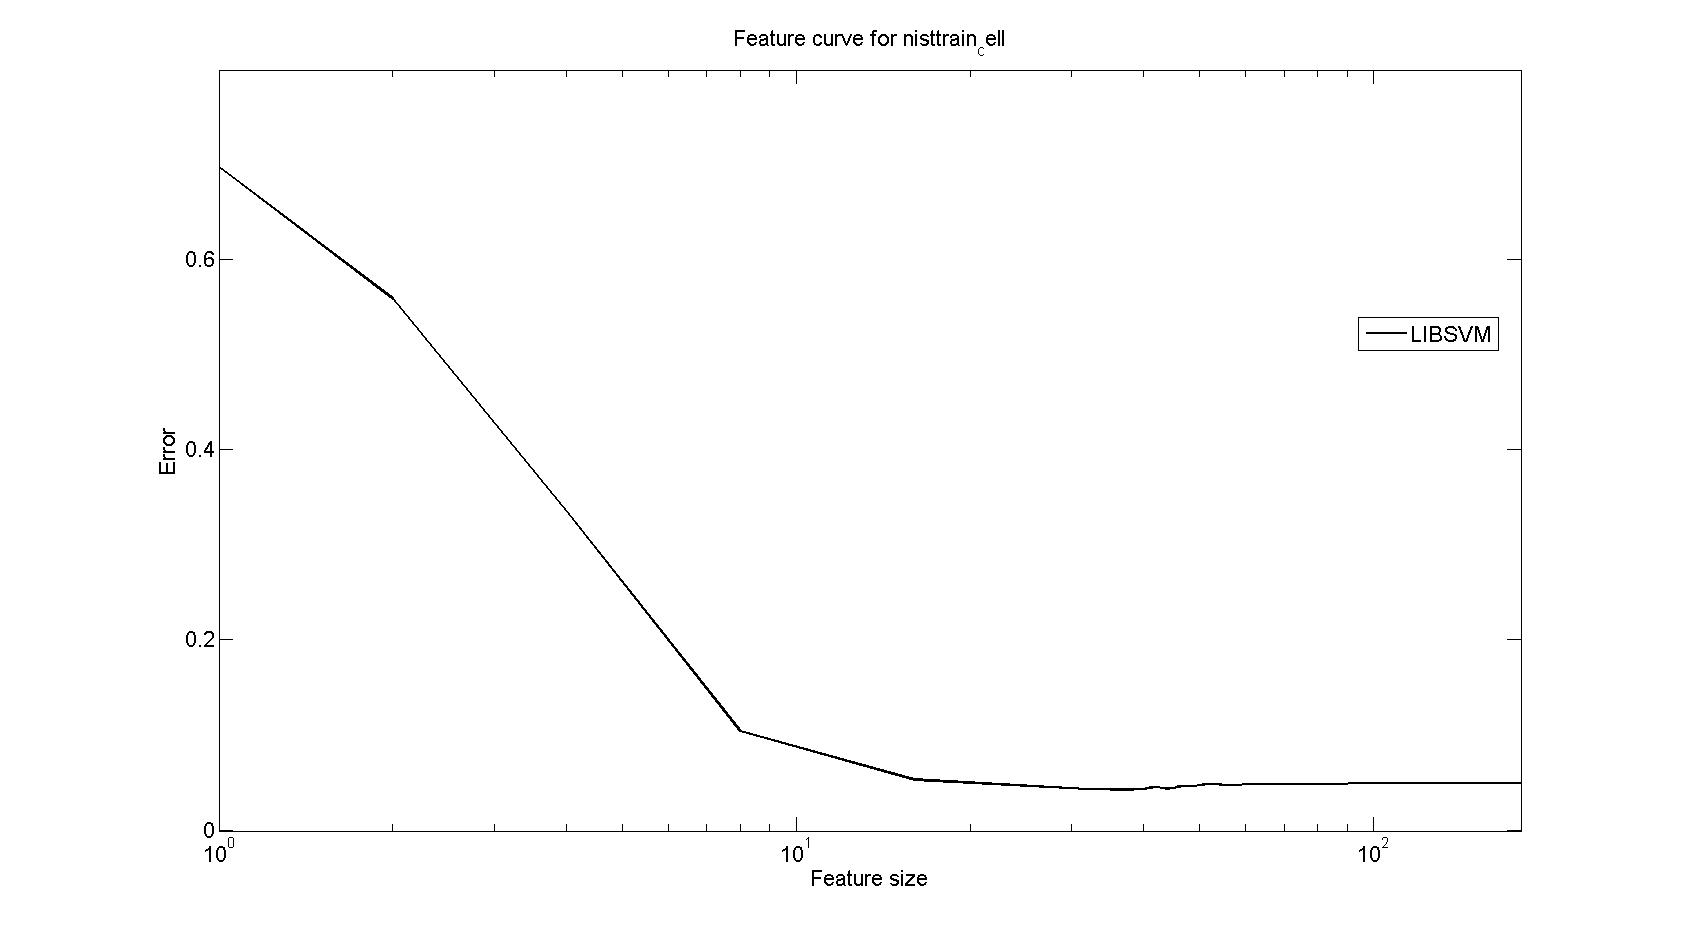
\includegraphics[trim = 25mm 10mm 25mm 20mm, clip,width=0.7\textwidth]{learningcurve-PCAmapped-data}
	\caption{Learning curve on PCA mapped data}
	\label{fig:learningcurve-PCAmapped-data}
\end{figure}

From the learning curve can be concluded that the best performance is obtained with at least $30$ dimensions. Surprisingly, the error-rate is hardly raising when more features are used. This may be caused by the big amount of training data compared to the total number of features. Looking in more detail to the outcome, it seems that a variability around $93 \%$, obtained with round about $43$ features, yields best results. 

For the test, the used classifiers are equal to the classifiers above to be able to compare the differences. For displaying purposes the results are not shown here but can be found in Appendix A, a summary of these results is shown in the table below.

\begin{table}[H]
  \small
  \centering
    \begin{tabular}{|l|llllll|l|}
    \hline
    \textbf{Bicubic} & 8x8   & 9x9   & 10x10 & 11x11 & 12x12 & 13x13 & Min \\
    \hline \hline
    PCA c-var & 0,034 & 0,029 & 0,036 & 0,035 & 0,034 & 0,039 & 0,029 \\
    PCA c-mean & 0,027 & 0,024 & 0,019 & 0,024 & 0,021 & 0,029 & 0,019 \\
    PCA domain & 0,025 & 0,026 & 0,023 & \textbf{0,017} & 0,023 & 0,028 & 0,017 \\
    PCA unscaled & 0,023 & 0,024 & 0,023 & 0,021 & 0,034 & 0,033 & 0,021 \\ 
    Pixels & 0,028 & 0,027 & 0,026 & 0,022 & 0,027 & 0,031 & 0,022 \\ \hline
		Minimum   & 0,023 & 0,024 & 0,019 & 0,017 & 0,021 & 0,028 & 0,017 \\
		\hline 
		\hline
    \textbf{Bilinear} & 8x8   & 9x9   & 10x10 & 11x11 & 12x12 & 13x13 & Min \\ \hline \hline
    PCA c-var & 0,032 & 0,033 & 0,037 & 0,041 & 0,038 & 0,033 & 0,032 \\
    PCA c-mean & 0,022 & 0,025 & 0,026 & 0,026 & 0,02  & 0,023 & 0,02 \\
    PCA domain & 0,025 & 0,025 & 0,029 & 0,024 & 0,019 & 0,025 & 0,019 \\
    PCA unscaled & 0,024 & \textbf{0,017} & 0,019 & 0,025 & 0,022 & 0,028 & 0,017 \\
    Pixels & 0,023 & 0,028 & 0,021 & 0,035 & 0,029 & 0,025 & 0,021 \\ \hline
		Minimum & 0,022 & 0,017 & 0,019 & 0,024 & 0,019 & 0,023 & 0,017 \\ 
    \hline
    \end{tabular}%
    \caption{Minimum error rates summary of all used classifiers after PCA per size, scaling method and mapping type} \label{table: error rate summary PCA}%
\end{table}%

\clearpage

The summary shows that in this case \textit{domain} scaling and no scaling at all perform best, but that \textit{c-mean} scaling is also performing well. It is surprising that classifying on the raw images gives an only little worse error rate. Besides the summary to show which scaling type performs best at which pixel size, also the performance of the classifiers will be shown per scaling type, neglecting the size of the images. 

\begin{table}[H]
  \small
  \centering
    \begin{tabular}{l|llllllllll|l}
    \hline
     & & & & & & & &  & \textbf{SVC P} & \textbf{SVC R} &  \\
          & \multicolumn{1}{l}{\textbf{parzen}} & \multicolumn{1}{l}{\textbf{ldc}} & \multicolumn{1}{l}{\textbf{qdc}} & \multicolumn{1}{l}{\textbf{fisher}} & \multicolumn{1}{l}{\textbf{nmc}} & \multicolumn{1}{l}{\textbf{knn}} & \multicolumn{1}{l}{\textbf{SVC P}} & \multicolumn{1}{l}{\textbf{SVC E}} & \textbf{(w=2)} & \textbf{(w=2.5)} & \multicolumn{1}{l}{\textbf{min}} \\ \hline
    PCA c-var & \multicolumn{1}{l}{0,041} & \multicolumn{1}{l}{0,093} & \multicolumn{1}{l}{0,044} & \multicolumn{1}{l}{0,121} & \multicolumn{1}{l}{0,164} & \multicolumn{1}{l}{0,035} & \multicolumn{1}{l}{0,052} & \multicolumn{1}{l}{0,237} & 0,029 & 0,324 & \multicolumn{1}{l}{0,029} \\
    PCA c-mean & \multicolumn{1}{l}{0,024} & \multicolumn{1}{l}{0,104} & \multicolumn{1}{l}{0,029} & \multicolumn{1}{l}{0,125} & \multicolumn{1}{l}{0,161} & \multicolumn{1}{l}{0,026} & \multicolumn{1}{l}{0,043} & \multicolumn{1}{l}{0,031} & 0,020  & 0,019 & \multicolumn{1}{l}{0,019} \\
    PCA domain & \multicolumn{1}{l}{0,028} & \multicolumn{1}{l}{0,098} & \multicolumn{1}{l}{0,03} & \multicolumn{1}{l}{0,135} & \multicolumn{1}{l}{0,173} & \multicolumn{1}{l}{0,032} & \multicolumn{1}{l}{0,035} & \multicolumn{1}{l}{0,031} & \textbf{0,017} & 0,021 & \multicolumn{1}{l}{0,017} \\
    PCA unscaled & \multicolumn{1}{l}{0,03} & \multicolumn{1}{l}{0,103} & \multicolumn{1}{l}{0,035} & \multicolumn{1}{l}{0,13} & \multicolumn{1}{l}{0,17} & \multicolumn{1}{l}{0,032} & \multicolumn{1}{l}{0,042} & \multicolumn{1}{l}{0,038} & 0,022 & 0,026 & \multicolumn{1}{l}{0,022} \\
    Pixels & \multicolumn{1}{l}{0,027} & \multicolumn{1}{l}{0,68} & \multicolumn{1}{l}{0,151} & \multicolumn{1}{l}{0,121} & \multicolumn{1}{l}{0,167} & \multicolumn{1}{l}{0,025} & \multicolumn{1}{l}{0,04} & \multicolumn{1}{l}{0,037} & 0,023 & 0,021 & \multicolumn{1}{l}{0,021} \\ \hline
    Min   & \multicolumn{1}{l}{0,024} & \multicolumn{1}{l}{0,093} & \multicolumn{1}{l}{0,029} & \multicolumn{1}{l}{0,121} & \multicolumn{1}{l}{0,161} & \multicolumn{1}{l}{0,025} & \multicolumn{1}{l}{0,035} & \multicolumn{1}{l}{0,031} & 0,017 & 0,019 & \multicolumn{1}{l}{0,017} \\
    \hline
    \end{tabular}%

  \caption{Minimum error rates of all sizes per classifier, scaling method and mapping type} \label{table: error rate summary PCA2}   
\end{table}% 

From the table we conclude that the support vector classifier for the \textit{polynomial} and \textit{radial kernel} perform best while using the scaling \textit{c-mean} and \textit{domain}. To show the performance of the classifiers on the PCA-mapped data, the confusion matrix is shown in Table~\ref{table: confusion matrix of PCA mapped data}.

\begin{table}[H]
  \centering
    \begin{tabular}{|c|llllllllll|l|}
    \hline
    \multicolumn{1}{|c|}{True} & \multicolumn{10}{c|}{\emph{Estimated labels}} & \\
    labels & 0     & 1     & 2     & 3     & 4     & 5     & 6     & 7     & 8     & 9     & Totals \\
    \hline
    0     & 198   & 0     & 0     & 1     & 0     & 0     & 0     & 0     & 1     & 0     & 200 \\
    1     & 0     & 198   & 0     & 0     & 1     & 0     & 0     & 0     & 0     & 1     & 200 \\
    2     & 0     & 0     & 198   & 1     & 0     & 0     & 0     & 1     & 0     & 0     & 200 \\
    3     & 1     & 0     & 0     & 196   & 0     & 1     & 0     & 0     & 2     & 0     & 200 \\
    4     & 0     & 0     & 0     & 0     & 200   & 0     & 0     & 0     & 0     & 0     & 200 \\
    5     & 1     & 1     & 0     & 0     & 1     & 196   & 0     & 0     & 1     & 0     & 200 \\
    6     & 0     & 0     & 1     & 0     & 0     & 0     & 199   & 0     & 0     & 0     & 200 \\
    7     & 0     & 0     & 0     & 0     & 0     & 0     & 0     & 198   & 0     & 2     & 200 \\
    8     & 1     & 0     & 1     & 0     & 0     & 0     & 0     & 0     & 196   & 2     & 200 \\
    9     & 0     & 0     & 0     & 0     & 0     & 0     & 0     & 0     & 0     & 200   & 200 \\
    \hline
    Totals & 201   & 199   & 200   & 198   & 202   & 197   & 199   & 199   & 200   & 205   & 2000 \\
    \hline
    \end{tabular}%
  \caption{Confusion matrix of PCA mapped data} \label{table: confusion matrix of PCA mapped data}%
\end{table}%

The confusion matrix is not showing particular wrong classified numbers, the errors seem to be randomly distributed.

\begin{comment}
\subsection{Classifying extra features with DIP image}

To optimize the classifier, we had the idea to compute more features because there is a big amount of test data. Therefore the \texttt{DIPimage} function was used, which can compute $26$ extra features out of the images. \texttt{DIPimage} is discussed more in-depth in the next section regarding scenario 2. The outcome of the classification over the features was performing a lot worse than direct classification on the pixels. Even when the size of the training data was lowered to avoid the \emph{curse of dimensionality}, it didn't get close to the already obtained results. The reason for the worse performance is probably the big available amount of training data which is enough to train complex classifiers on just the pixels. More about extracting features in scenario 2.
\end{comment}

\subsection{Optimizing Results}

The obtained error-rates in this chapter show that classification on raw pixels using PCA yields the lowest error rate. Until this point, only square image sizes were used. Because the drawings are not squares we will try to optimize the error rate by trying different pixel sizes. By resizing to other sizes, it could happen that more useful pixels may be saved and the less useful could be filtered away. All combinations between $8 \times 8$ and $13 \times 13$ are computed for the different classifiers and scale-interpolations, therefore not all the results will be shown. The minimum error rates for all the mentioned sizes over all classifiers are shown per interpolation method (\textit{nearest} is already skipped here) in Appendix A (Table~\ref{table: minimum error rates all sizes}). \\

In conclusion of the results, the SVC classifier has the best performance for the polynomial kernel with adapted weight when using the bicubical interpolated pixels with size $10 \times 13$. There is no scaling used and the data is mapped with PCA. However, the results vary per session and vary even more when using them on the \textit{nist$\_$eval} dataset. It seems that the best settings differ per training and testset and that this is the phase of fine-tuning. Error rates between $1.0\%$ and $1.8\%$ are obtained when testing directly on the (randomly sampled) \texttt{nist$\_$data}. The performance when using \texttt{nist$\_$eval} is little worse with error rates around $2.0\%$. 

\section{Scenario 2: \textit{System is trained for each batch}}

The second scenario allows the classifier to be trained for every batch of cheques to be processed. As a concequence the dataset available for training is much smaller, in this scenario we train the classifier using at most $10$ objects per class. The target for this assignment is $25\%$ test error.

\subsection{Representation}
Again the development of our algorithm begins with choosing the best representation for our data set. Here we need to take into account that the number of objects that are available for training is small compared to the first scenario. Therefore the information in the raw pixel features as were used in the first part is probably not sufficient. We are left with two options, calculate various \emph{image features} or choose the path of \emph{dissimilarity measures}. In addition to the pixel features we decided to calculate image features. The advantage over the image feature representation is that every aspect of the digits can be calculated. \\

The standard methods of Matlab supplemented with the \texttt{PRtools} are limited in the image analysis field. By deciding upon using the image feature representation a flexible and powerful image processing toolkit is required. We have chosen to incorporate \texttt{DIPimage} for our project since we already had experience with it and integrates nicely with \texttt{PRtools}.

\subsection{Image Features}

After converting our images to \texttt{DIPimage} objects we can exploit the \texttt{measurement} method that allows easy computation of a large amount of image statistics and more. We have selected a large amount of these statistics to use as features. In the selection process we have intuitively picked the features which we thought are differentiating the digits. Table~\ref{table:image-features} lists the features that were initially used as features. We have used $16$ different image features types, however these make a total of $25$ features since some of these feature types contain an $x$ and $y$ coordinate (center) or a minimum and maximum value (Feret).

\begin{table}[H]
    \small
	\centering
    \begin{tabular}{|l|l|}
    \hline
    \textbf{Feature} & \textbf{Description} \\
    \hline
    \emph{Object Count}     & Number of objects, sometimes there are two smaller objects \\
    \emph{Total Size}       & Total number of object pixels           \\
    \emph{Radius}       	& Statistics on the radius using chain-code method           \\
    \emph{Center}  		& Coordinates of the geometric mean \\
    \emph{Gravity} 		& Coordinates of the center-of-mass \\
    \emph{Inertia} 		& Moments of intertia \\
    \emph{Mu} 				& Elements of the inertia tensor \\
    \emph{ConvexArea} 		& Area of the convex hull \\
    \emph{CartesianBox} 	& Cartesian box size around the object \\
    \emph{CCBendingEnergy} & Bending energy of the object perimeter \\
    \emph{Convexity} 		& Area fraction of convex hull covered by the object \\
    \emph{Feret} 			& Minimum and maximum object diameters \\
    \emph{Mean} 			& Mean object intensity \\
    \emph{Circularity} 	& Circularity of the object \\
    \emph{Perimeter} 		& Length of the object perimeter (chain-code) \\
    \emph{Sum of Pixels} 	& Sum of object intensity (mass) \\
    \hline
    \end{tabular}
    \caption{Image features computed by DIPimage's \texttt{measurement} function \label{table:image-features}}
\end{table}

To be able to compute all these features we create two image objects in Matlab; the original image and a thresholded binary image. The binary image is required for measuring some of the above features. After measuring all the features we build a matrix containg the results, this will become our dataset. The Matlab code for computing the dataset is given in Appendix B (Listing~\ref{code:myrep2}).

\subsection{Initial Results and Optimal Classifier}

Having obtained the feature matrix and converted this to data set we did some initial testing on the features. We loaded the entire NIST dataset and generated a random dataset with $10$ objects per class for training purpose. We evaluated the performance of the classifiers using the \texttt{nist\_eval} function. The complete script that was used for performance evaluation is given in Appendix B in code Listing~\ref{code:eval-script-scenario}. \\

We started training with various classifiers; \emph{nearest-mean}, \emph{fisher}, \emph{parzen}, \emph{k-nearest neighbor} and \emph{support vector machines}. The training and test phase with the class sizes as stated above were repeated five times in order to get representative results, our foundings are listed in Table~\ref{table:results-only-features}. For each result the best performance (lowest error) is indicated in bold. 

\begin{table}[H]
	\centering
    \begin{tabular}{|l|llllll|}
    \hline
	& \textbf{1NN} & \textbf{3NN} & \textbf{Parzen} & \textbf{NMC} & \textbf{Fisher} & \textbf{SVC} \\
	\hline
1 & 0.5920    & 0.5160    & 0.5820    & 0.7780 & \textbf{0.2160}   & 0.2260 \\
2 & 0.5820    & 0.4840    & 0.5720    & 0.7080 & \textbf{0.2160}   & 0.2300 \\
3 & 0.6140    & 0.5520    & 0.5900    & 0.7240 & 0.1920   & \textbf{0.1840} \\
4 & 0.5980    & 0.5120    & 0.6560    & 0.7020 & \textbf{0.2500}   & 0.3040 \\
5 & 0.6220    & 0.5620    & 0.7240    & 0.7080 & \textbf{0.1820}   & 0.3040 \\
	\hline
    \end{tabular}
    \caption{Error rates of various classifiers using $25$ image features \label{table:results-only-features}}
\end{table}

\clearpage

From these measurements we directly notice that using the Fisher classifier yields the best result with an average error rate of $21.1\%$. Although this is a good initial result, we want to decrease the error rate by adding some improvements. In the next section we continue tests using Fisher and support-vector machines classifiers since these give the best initial results.

\subsection{Improving the Error Rate}

To improve the classification accuracy we wanted to try adding more features to the dataset returned by the \texttt{my\_rep} function. In order to do this, two options were available to us, first we could compute more (advanced) image features, and second we could down-scale the images and add the pixel values as features. Since we already maximally exploited DIPimage's \texttt{measure} function to compute image features we chose to test the second method first. \\

The \texttt{my\_rep} function was modified so that it also down-scales the image to square size of $d \times d$ pixels. Before doing this we applied \emph{gaussian smoothing} to the digits and then applied resampling using \emph{Lanczos method} \cite{lanczos-filtering} as implemented by DIPimage. Our approach is to start by down-scaling the image by a large factor (small $d$) so that little pixels are added as features. We perform classification using Fisher and SVC classifiers since these initially gave the best results. Then we continue gradually increasing $d$ and see what effect this has on the error rate. The results are summarized in the graph displayed in Figure~\ref{fig:error-rate-increasing-pixel-features}, the error rates of Fisher are shown as dashed line while the SVC results are represented by the solid line.

\begin{figure}[H]
    \center
    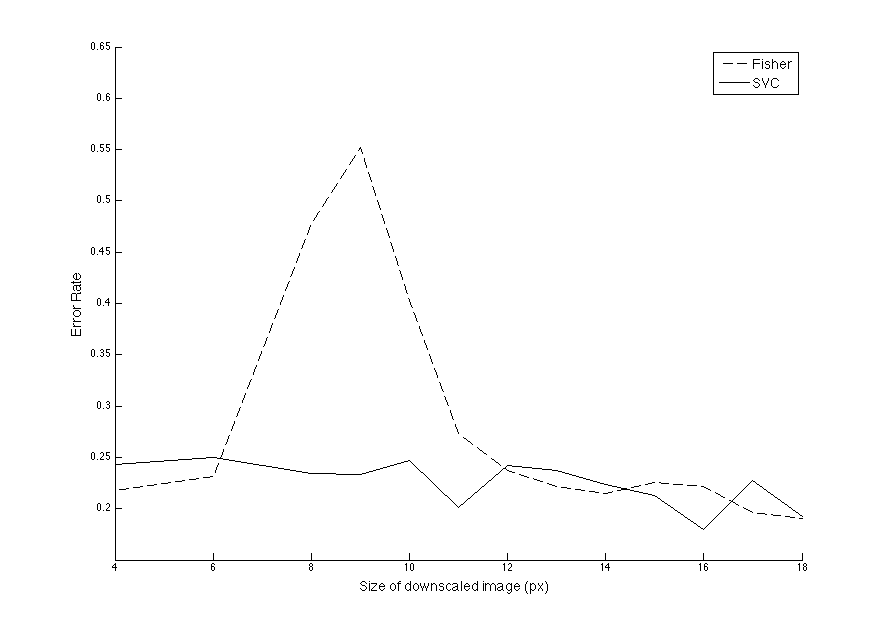
\includegraphics[trim = 25mm 10mm 25mm 10mm, clip,width=.8\textwidth]{scenario2-adding-pixels.png}
    \caption{Error rate with adding increasing number of pixel (average over $4$ tests) \label{fig:error-rate-increasing-pixel-features}}
\end{figure}

\clearpage

The figure above shows the average error rate over $4$ tests. Strangely enough we observed a very high average error rate for the Fisher classifier when the down-scaled image dimensions were approximately $9 \times 9$ pixels. This increased error rate did not occur for SVC, we are not sure why this occurs for Fisher. The lowest error rate of $\mathbf{18 \%}$ was observed using the support-vector classifier with a down-scaled image at $16 \times 16$ pixels. 

\subsection{Feature Selection}

We also tested our classifier after performing \emph{feature selection} using the \texttt{featselb} function. As a starting point we choose the optimal settings from our previous experiment, i.e. we used $25$ image features and $16 \times 16$ additional pixel features. Unfortunately a decrease in error rate was not observed and the computation times for performing feature selection on an initial number of $25 + 16^2 = 281$ were too long. The Matlab code that was used for performing feature selection can be found in Listing~\ref{code:scenario2-test-featsel} (Appendix B).

\subsection{Feature Extraction}

Since feature selection did not give the desired results we continued by performing feature extracting by means of PCA. Just like in scenario 1 we first computed the scaled mapping with \texttt{scalem} and then the PCA mapping with \texttt{pcam}. These mappings were saved in our test script and multiplied with the SVC classifier that was trained on our dataset. For these tests we only used SVC as classifier and included the pixel features in the data set. The error rates obtained after training the classifier on $10$ objects per class are displayed in Table~\ref{table:scenario2-pca}. Using PCA we were not able to decrease the misclassifation rate below the $\mathbf{18 \%}$ that was initially achieved.

\begin{table}[H]
    \centering
    \begin{tabular}{l|lll|}
    \hline
    Dimensions & \textbf{15}     & \textbf{40}     & \textbf{60}     \\ \hline
    \textbf{1}          & 0.1900 & 0.2260 & 0.2720 \\ 
    \textbf{2}          & 0.1940 & 0.3020 & 0.2300 \\
    \textbf{3}          & 0.1940 & 0.2560 & 0.2600 \\
    \textbf{4}          & 0.3380 & 0.2080 & 0.1820 \\ \hline
    Average   & 0.2290 & 0.2480 & 0.2360 \\ \hline
    \end{tabular}
    \caption{Error rates after performing PCA on the initial dataset of $281$ features. \label{table:scenario2-pca}}
\end{table}

\section{Recommendations}

In this section we discuss possible improvements for the classifiers we presented in this article. In the first scenario we noticed that there is a lot of variance in the performance of the classifiers, the classifiers are not dealing well with the most extreme variations in the dataset. Confusion matrix on Page~\pageref{table: confusion matrix of PCA mapped data} shows that mistakes are made randomly, probably caused by a really bad handwriting. Besides that, we saw at the learning curve that we are not suffering from the \emph{curse of dimensionality}. \\

Taking these points into account, more features could be added or the classification could be made more complex without the immediate risk of overtraining. To make the classifier less sensitive for variation, different classifiers could be combined, because they can react different on extreme variations. Combining classifiers that react different on variation could be powerful and could be even better by inserting a reject classification. Extra computed features could be less sensitive to certain kinds of variation in the handwriting, therefore features could be added to the pixels as contributing extra features. The new feature space should be mapped with PCA to extract correlations.\\

The last recommendation for the first scenario, is to improve the images before mapping and classifying them. There are a lot of techniques available to improve the quality of images or to adapt images to be able to extract important information more easy. Other useful techniques could be to turn the pictures and cut the useless pixels. \\

Also we discuss the possibilities for improving the algorithm for the second scenario. For this scenario there are two possible ways to improve the classifier. First the accuracy of the classifier can be increased, whereas the second enhancement focusses on computing time. For improving the error rates adding more pixel features is not the way to go as the results in Figure~\ref{fig:error-rate-increasing-pixel-features} shows. We recommend using less pixel values but select them more carefully by calculating which pixels contain most information. This can be done by incorporating the \emph{Shannon entropy} of the pixels and selecting the ones that are most valuable. Another approach would be to extend the preprocessing steps. Morphological image operations such as \emph{opening} and \emph{closing} can help to make the written digits more clear allowing easier recognition. \\

To better understand the classification results we also recommend in-depth analysis of the \emph{confusion matrix} or the misclassification rates per individual digit. This allows for better understanding of the results and possible ways to improve the algorithm by implementing image features that are robust for the digits that are currently hard to classify. For the classifier we designed for scenario 2 the digit `eight' was the most problematic as can be seen from Figure~\ref{fig:digit-misclassification} (note: these error rates were not obtained using \texttt{nist\_eval}). Analysing these results and coming up with new features that are better capable to recognise the digit $8$ for example was beyond the scope of this project but can be very interesting for future work.

\begin{figure}[H]
    \center
    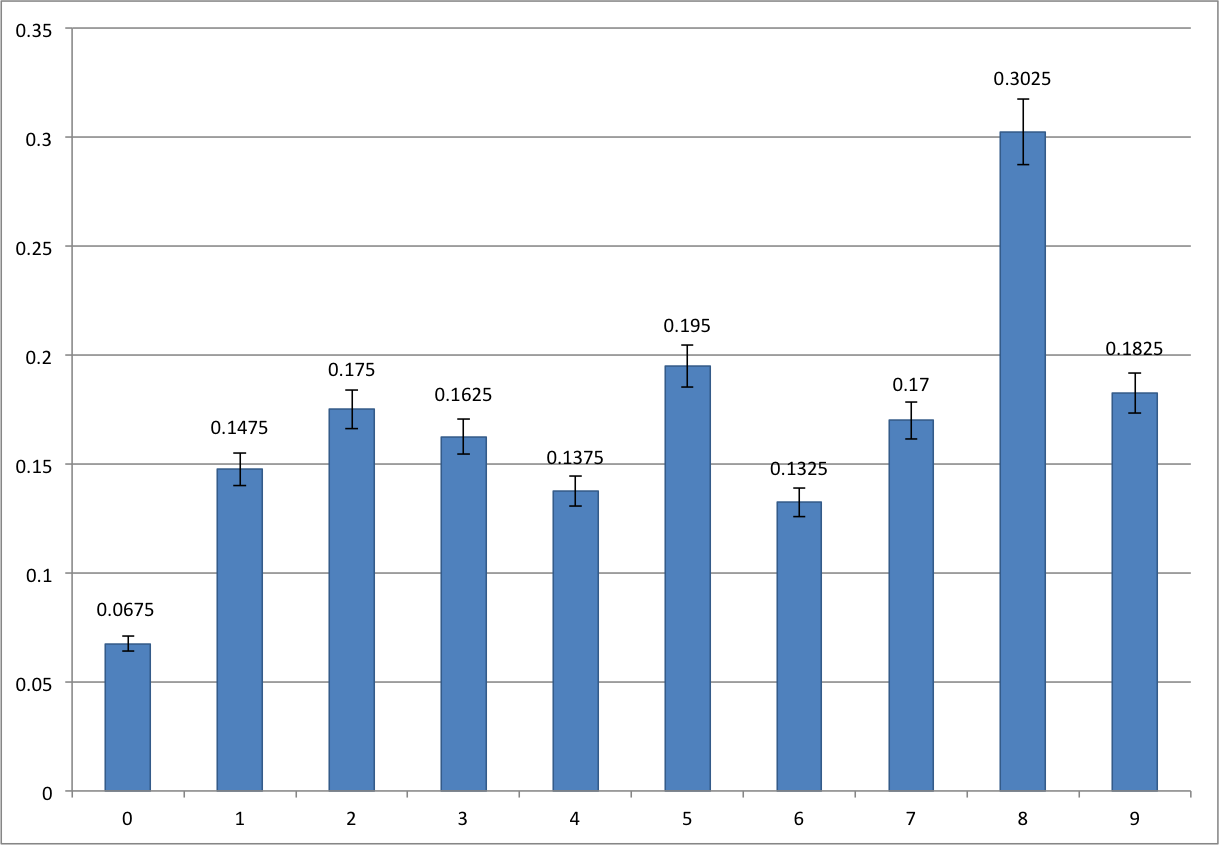
\includegraphics[width=.7\textwidth]{misclassification-digits}
    \caption{Misclassification rates per digit (average over $8$ batches) \label{fig:digit-misclassification}}
\end{figure}

\clearpage

\section{Appendix A: Result matrices}

The matrix of the error-rates after applying different classifiers on PCA-mapped images and on raw pixels is shown below. The resizing is only done for scale $8 \times 8$ until $13 \times 13$ for bilinear and cubical interpolation of pixels, because the best results are gotten for these settings. The lowest error-rate is written in bold.

\begin{table}[H]
  \small
  \centering
    \begin{tabular}{l|l|llllllllll|l|}
    \hline
    \textbf{size} & \textbf{PCA-mapping} & \textbf{parzen} & \textbf{ldc} & \textbf{qdc} & \textbf{fisher} & \textbf{nmc} & \textbf{knnc} & \textbf{svc p} & \textbf{svc e} & \textbf{svc p2} & \textbf{svc r2.5} & \textbf{min} \\
    \hline \hline
    8x8   & PCA c-var & 0,041 & 0,115 & 0,052 & 0,152 & 0,21  & 0,047 & 0,052 & 0,249 & 0,034 & 0,324 & 0,034 \\
          & PCA c-mean & 0,032 & 0,106 & 0,034 & 0,125 & 0,162 & 0,033 & 0,047 & 0,035 & 0,03  & 0,027 & 0,027 \\
          & PCA domain & 0,043 & 0,106 & 0,039 & 0,135 & 0,195 & 0,049 & 0,049 & 0,035 & 0,025 & 0,029 & 0,025 \\
          & PCA pixels & 0,037 & 0,107 & 0,045 & 0,139 & 0,19  & 0,04  & 0,044 & 0,038 & 0,028 & 0,028 & 0,028 \\
          & pixels & 0,036 & 0,68  & 0,151 & 0,141 & 0,181 & 0,032 & 0,043 & 0,037 & 0,023 & 0,026 & 0,023 \\ \hline
    9x9   & PCA c-var & 0,043 & 0,097 & 0,044 & 0,121 & 0,195 & 0,035 & 0,053 & 0,237 & 0,029 & 0,358 & 0,029 \\
          & PCA c-mean & 0,032 & 0,125 & 0,042 & 0,163 & 0,209 & 0,027 & 0,053 & 0,039 & 0,024 & 0,028 & 0,024 \\
          & PCA domain & 0,045 & 0,13  & 0,041 & 0,157 & 0,193 & 0,045 & 0,052 & 0,045 & 0,026 & 0,031 & 0,026 \\
          & PCA pixels & 0,032 & 0,12  & 0,042 & 0,153 & 0,202 & 0,034 & 0,051 & 0,04  & 0,031 & 0,027 & 0,027 \\
          & pixels & 0,031 & 0,887 & 0,491 & 0,121 & 0,167 & 0,032 & 0,042 & 0,039 & 0,032 & 0,024 & 0,024 \\ \hline
    10x10 & PCA c-var & 0,048 & 0,11  & 0,065 & 0,142 & 0,203 & 0,048 & 0,066 & 0,26  & 0,036 & 0,453 & 0,036 \\
          & PCA c-mean & 0,024 & 0,104 & 0,029 & 0,127 & 0,187 & 0,026 & 0,043 & 0,031 & 0,02  & 0,019 & 0,019 \\
          & PCA domain & 0,034 & 0,098 & 0,03  & 0,135 & 0,173 & 0,036 & 0,035 & 0,031 & 0,023 & 0,023 & 0,023 \\
          & PCA pixels & 0,034 & 0,103 & 0,041 & 0,13  & 0,17  & 0,032 & 0,046 & 0,043 & 0,026 & 0,03  & 0,026 \\
          & pixels & 0,032 & 0,9   & 0,654 & 0,122 & 0,188 & 0,036 & 0,04  & 0,04  & 0,025 & 0,023 & 0,023 \\ \hline
    11x11 & PCA c-var & 0,043 & 0,097 & 0,054 & 0,129 & 0,164 & 0,039 & 0,063 & 0,356 & 0,035 & 0,508 & 0,035 \\
          & PCA c-mean & 0,033 & 0,109 & 0,034 & 0,136 & 0,161 & 0,035 & 0,048 & 0,046 & 0,031 & 0,024 & 0,024 \\
          & PCA domain & 0,028 & 0,119 & 0,035 & 0,151 & 0,183 & 0,035 & 0,047 & 0,031 & \textbf{0,017} & 0,021 & \textbf{0,017} \\
          & PCA pixels & 0,03  & 0,105 & 0,035 & 0,147 & 0,195 & 0,032 & 0,042 & 0,039 & 0,022 & 0,026 & 0,022 \\
          & pixels & 0,027 & 0,9   & 0,682 & 0,136 & 0,185 & 0,025 & 0,049 & 0,05  & 0,023 & 0,021 & 0,021 \\ \hline
    12x12 & PCA c-var & 0,056 & 0,111 & 0,061 & 0,141 & 0,191 & 0,055 & 0,071 & 0,395 & 0,034 & 0,578 & 0,034 \\
          & PCA c-mean & 0,038 & 0,106 & 0,036 & 0,126 & 0,186 & 0,043 & 0,049 & 0,041 & 0,021 & 0,024 & 0,021 \\
          & PCA domain & 0,033 & 0,101 & 0,039 & 0,14  & 0,196 & 0,032 & 0,049 & 0,033 & 0,026 & 0,023 & 0,023 \\
          & PCA pixels & 0,039 & 0,122 & 0,035 & 0,159 & 0,178 & 0,043 & 0,058 & 0,044 & 0,033 & 0,027 & 0,027 \\
          & pixels & 0,051 & 0,9   & 0,703 & 0,136 & 0,188 & 0,053 & 0,062 & 0,064 & 0,034 & 0,041 & 0,034 \\ \hline
    13x13 & PCA c-var & 0,052 & 0,093 & 0,054 & 0,131 & 0,191 & 0,051 & 0,065 & 0,424 & 0,039 & 0,625 & 0,039 \\
          & PCA c-mean & 0,042 & 0,128 & 0,037 & 0,151 & 0,195 & 0,038 & 0,064 & 0,046 & 0,03  & 0,029 & 0,029 \\
          & PCA domain & 0,045 & 0,108 & 0,03  & 0,145 & 0,181 & 0,052 & 0,054 & 0,051 & 0,028 & 0,028 & 0,028 \\
          & PCA pixels & 0,045 & 0,13  & 0,048 & 0,161 & 0,203 & 0,044 & 0,063 & 0,058 & 0,031 & 0,035 & 0,031 \\
          & pixels & 0,044 & 0,899 & 0,699 & 0,134 & 0,176 & 0,044 & 0,056 & 0,072 & 0,033 & 0,044 & 0,033 \\ \hline
          & min & 0,024 & 0,093 & 0,029 & 0,121 & 0,161 & 0,025 & 0,035 & 0,031 & \textbf{0,017} & 0,019 & 0,017 \\
    \hline
    \end{tabular}%
		\caption{Error rates on PCA mapped and raw pixels for bicubic interpolation between pixels}  \label{table: errorrates of PCA mappings bicubic}%
\end{table}%

% Table generated by Excel2LaTeX from sheet 'Sheet1'
\begin{table}[H]
  \small
  \centering
    \begin{tabular}{l|l|llllllllll|l|}
    \hline
    \textbf{size} & \textbf{PCA-mapping} & \textbf{parzen} & \textbf{ldc} & \textbf{qdc} & \textbf{fisher} & \textbf{nmc} & \textbf{knnc} & \textbf{svc p} & \textbf{svc e} & \textbf{svc p2} & \textbf{svcr2.5} & \textbf{min} \\
    \hline \hline
    8x8   & PCA c-var & 0,032 & 0,109 & 0,05  & 0,143 & 0,197 & 0,033 & 0,065 & 0,265 & 0,034 & 0,328 & 0,032 \\
          & PCA c-mean & 0,037 & 0,119 & 0,034 & 0,14  & 0,204 & 0,039 & 0,044 & 0,037 & 0,022 & 0,023 & 0,022 \\
          & PCA domain & 0,03  & 0,115 & 0,046 & 0,142 & 0,184 & 0,043 & 0,049 & 0,031 & 0,025 & 0,025 & 0,025 \\
          & PCA pixels & 0,033 & 0,098 & 0,042 & 0,128 & 0,184 & 0,034 & 0,036 & 0,025 & 0,025 & 0,024 & 0,024 \\
          & pixels & 0,03  & 0,801 & 0,265 & 0,114 & 0,146 & 0,033 & 0,04  & 0,027 & 0,027 & 0,023 & 0,023 \\ \hline
    9x9   & PCA c-var & 0,04  & 0,109 & 0,04  & 0,139 & 0,189 & 0,039 & 0,065 & 0,28  & 0,033 & 0,37  & 0,033 \\
          & PCA c-mean & 0,039 & 0,109 & 0,044 & 0,125 & 0,19  & 0,043 & 0,049 & 0,037 & 0,033 & 0,025 & 0,025 \\
          & PCA domain & 0,032 & 0,089 & 0,034 & 0,11  & 0,161 & 0,031 & 0,039 & 0,034 & 0,025 & 0,026 & 0,025 \\
          & PCA pixels & 0,031 & 0,098 & 0,033 & 0,126 & 0,16  & 0,035 & 0,035 & 0,026 & 0,02  & \textbf{0,017} & \textbf{0,017} \\
          & pixels & 0,044 & 0,893 & 0,547 & 0,143 & 0,181 & 0,043 & 0,043 & 0,035 & 0,036 & 0,028 & 0,028 \\ \hline
    10x10 & PCA c-var & 0,053 & 0,121 & 0,057 & 0,147 & 0,214 & 0,052 & 0,074 & 0,28  & 0,037 & 0,47  & 0,037 \\
          & PCA c-mean & 0,031 & 0,122 & 0,051 & 0,159 & 0,182 & 0,033 & 0,055 & 0,035 & 0,028 & 0,026 & 0,026 \\
          & PCA domain & 0,029 & 0,123 & 0,035 & 0,154 & 0,183 & 0,029 & 0,048 & 0,042 & 0,029 & 0,031 & 0,029 \\
          & PCA pixels & 0,029 & 0,102 & 0,031 & 0,137 & 0,178 & 0,036 & 0,045 & 0,036 & 0,021 & 0,019 & 0,019 \\
          & pixels & 0,036 & 0,896 & 0,705 & 0,126 & 0,153 & 0,037 & 0,037 & 0,034 & 0,026 & 0,021 & 0,021 \\ \hline
    11x11 & PCA c-var & 0,05  & 0,112 & 0,046 & 0,142 & 0,197 & 0,048 & 0,061 & 0,362 & 0,041 & 0,529 & 0,041 \\
          & PCA c-mean & 0,042 & 0,112 & 0,044 & 0,145 & 0,187 & 0,045 & 0,05  & 0,04  & 0,026 & 0,026 & 0,026 \\
          & PCA domain & 0,029 & 0,098 & 0,04  & 0,122 & 0,166 & 0,035 & 0,042 & 0,035 & 0,026 & 0,024 & 0,024 \\
          & PCA pixels & 0,037 & 0,119 & 0,041 & 0,146 & 0,191 & 0,035 & 0,049 & 0,037 & 0,026 & 0,025 & 0,025 \\
          & pixels & 0,043 & 0,9   & 0,716 & 0,162 & 0,194 & 0,043 & 0,049 & 0,055 & 0,035 & 0,035 & 0,035 \\ \hline
    12x12 & PCA c-var & 0,056 & 0,129 & 0,064 & 0,16  & 0,219 & 0,058 & 0,083 & 0,424 & 0,038 & 0,591 & 0,038 \\
          & PCA c-mean & 0,028 & 0,111 & 0,035 & 0,149 & 0,179 & 0,035 & 0,045 & 0,042 & 0,02  & 0,02  & 0,02 \\
          & PCA domain & 0,035 & 0,118 & 0,045 & 0,151 & 0,189 & 0,046 & 0,043 & 0,041 & 0,019 & 0,024 & 0,019 \\
          & PCA pixels & 0,03  & 0,113 & 0,039 & 0,144 & 0,193 & 0,028 & 0,046 & 0,042 & 0,022 & 0,024 & 0,022 \\
          & pixels & 0,043 & 0,899 & 0,744 & 0,142 & 0,174 & 0,042 & 0,051 & 0,048 & 0,034 & 0,029 & 0,029 \\ \hline
    13x13 & PCA c-var & 0,034 & 0,112 & 0,053 & 0,148 & 0,2   & 0,041 & 0,072 & 0,416 & 0,033 & 0,62  & 0,033 \\
          & PCA c-mean & 0,023 & 0,113 & 0,035 & 0,145 & 0,188 & 0,028 & 0,047 & 0,04  & 0,023 & 0,023 & 0,023 \\
          & PCA domain & 0,032 & 0,103 & 0,031 & 0,13  & 0,18  & 0,039 & 0,048 & 0,044 & 0,031 & 0,025 & 0,025 \\
          & PCA pixels & 0,034 & 0,113 & 0,048 & 0,148 & 0,179 & 0,039 & 0,046 & 0,042 & 0,029 & 0,028 & 0,028 \\
          & pixels & 0,037 & 0,9   & 0,733 & 0,114 & 0,154 & 0,037 & 0,053 & 0,043 & 0,025 & 0,026 & 0,025 \\ \hline
          & min   & 0,023 & 0,089 & 0,031 & 0,11  & 0,146 & 0,028 & 0,035 & 0,025 & 0,019 & \textbf{0,017} & 0,017 \\
    \hline
    \end{tabular}%
		  \caption{Error rates on PCA mapped and raw pixels for bilinear interpolation between pixels}   \label{table: errorrates of PCA mappings bilinear}%
\end{table}%

\clearpage

\begin{table}[H]
  \centering  
    \begin{tabular}{|l|ll|} \hline
    \textbf{size} & \textbf{bicubic} & \textbf{bilinear} \\ \hline \hline
    8x8   & 0,018 & 0,021 \\
    9x8   & 0,019 & 0,022 \\
    10x8  & 0,02  & 0,016 \\
    11x8  & 0,014 & 0,02 \\
    12x8  & 0,025 & 0,018 \\
    13x8  & 0,02  & 0,023 \\
    8x9   & 0,022 & 0,02 \\
    9x9   & 0,018 & 0,024 \\
    10x9  & 0,018 & 0,022 \\
    11x9  & 0,018 & 0,018 \\
    12x9  & 0,018 & 0,021 \\
    13x9  & 0,018 & 0,018 \\
    8x10  & 0,014 & 0,027 \\
    9x10  & 0,018 & 0,018 \\
    10x10 & 0,02  & 0,022 \\
    11x10 & 0,018 & 0,021 \\
    12x10 & 0,018 & 0,019 \\
    13x10 & 0,021 & 0,018 \\
    8x11  & 0,02  & 0,022 \\
    9x11  & 0,015 & 0,023 \\
    10x11 & 0,02  & 0,021 \\
    11x11 & 0,02  & 0,021 \\
    12x11 & 0,02  & 0,022 \\
    13x11 & 0,021 & \textbf{0,014} \\
    8x12  & 0,02  & 0,019 \\
    9x12  & 0,017 & 0,023 \\
    10x12 & 0,016 & 0,017 \\
    11x12 & 0,021 & 0,024 \\
    12x12 & 0,022 & 0,019 \\
    13x12 & 0,017 & 0,023 \\
    8x13  & 0,016 & 0,016 \\
    9x13  & 0,019 & 0,017 \\
    10x13 & \textbf{0,01} & 0,021 \\
    11x13 & 0,023 & \textbf{0,014} \\
    12x13 & 0,017 & 0,02 \\
    13x13 & 0,022 & 0,015 \\
    \hline
    min   & 0,01  & 0,014 \\
		\hline
    \end{tabular}%
  \caption{minimum error rates of all used classifiers per pixelsize} \label{table: minimum error rates all sizes}%
\end{table}%
 
\clearpage

\section{Appendix B: Matlab Code}

\begin{lstlisting}[caption=Script for performance evaluation,label=code:eval-script-scenario]
nist_data = prnist(0:9,1:1000);

iter = 2;       % Number of performance evaluations
num_test = 50;  % Number of test objects per class

errors = zeros(1:iter, 1);

for i = 1:iter
    % Generate a random training set with 10 objects per class 
    n_trn = gendat(nist_data, 0.01);
    % Calculate trainings prdataset object
    trn = my_rep2(n_trn);
    
    % Train SVC classifier
    w = svc(trn);
    
    % Evaluate performance of classifier
    E = nist_eval('my_rep2', w, num_test);
    
    errors(i) = E;
end

disp(errors);
\end{lstlisting}

\begin{lstlisting}[caption=Script for performance evaluation with feature selection,label=code:scenario2-test-featsel]
for i = 1:iter
    % Generate a random training set with 10 objects per class 
    n_trn = gendat(nist_data, 0.01);
    % Calculate trainings prdataset object

    trn_unselected = my_rep2(n_trn);

    [mapping, R] = featself(trn_unselected);

    trn_featsel = trn_unselected*mapping;

    % Train SVC classifier
    %w_fisher = fisherc(trn_featsel);
    w_svc = svc(trn_featsel);
    
    %w_fisher_map = mapping*w_fisher;
    w_svc_map = mapping*w_svc;
    
    %E1 = nist_eval('my_rep2', w_fisher_map, num_test);
    E2 = nist_eval('my_rep2', w_svc_map, num_test);
    
    %errors(i,1) = E1;   % Fisher
    errors(i,1) = E2;   % SVC
end
\end{lstlisting}

\begin{lstlisting}[caption=Computation of the dataset for Scenario 2, label=code:myrep2]
function a = my_rep2( m )

    % Simple preprocessing
    m = m*im_resize([],[128 128])*im_box([],1,0);

    % Pixel features of size d*d
    d = 16; 
    
    % Converting to DIPimage and computing pixel features
    % Empty matrix for the results
    M = zeros(length(m), d^2 + 25);
    
    % Obtain the label from the object
    labels = getlabels(m);

    for i = 1:length(m)
        % Convert to DIPimage object
        dip_img = data2im(m(i));

        % Perform closing operation on the image
        %dip_img = closing(dip_img, 10);
        %dip_img = smooth(dip_img, 4);
        
        % Perform gray-value stretching
        %dip_img = stretch(dip_img);

        % Threshold the image to obtain binary represtation
        binary = threshold(dip_img);
        msr = measure(binary, dip_img, ({'Size','Radius', 'Inertia', 'Mu', 'ConvexArea', 'Center', 'Gravity','CartesianBox','Perimeter','Feret','P2A','Convexity','Sum','Mean','CCBendingEnergy','MajorAxes'}));

        % Default we set it to the first object
        j = 1;

        obj_count = size(msr, 1);

        % Some threshold measures have multiple entries since there
        % are multiple objects. However the first one is also the largest
        if (obj_count ~= 1)
            % More than one object in the image
            % We select on the largest object
            [val, j] = max(msr.Size);
            %fprintf('Multiple objects found in object %i with label %i...\n', i, numlab);

            % Selected with the max size has index j
        end
        
        M(i,1)  = obj_count;         % number of objects
        M(i,2)  = sum(msr.Size);     % size of all objects
        M(i,3)  = msr.Radius(2,j);   % avg. radius of largest object
        M(i,4)  = msr.Center(1,j);   % CenterX of largest object
        M(i,5)  = msr.Center(2,j);   % CenterY of largest object
        M(i,6)  = msr.Gravity(1,j);  % GravityX of largest object
        M(i,7)  = msr.Gravity(2,j);  % GravityY of largest object
        M(i,8)  = msr.Inertia(1,j);  % InertiaM1 of largest object
        M(i,9)  = msr.Inertia(2,j);  % InertiaM2 of largest object
        M(i,10) = msr.Mu(1,j);       % Mu_xx of largest object
        M(i,11) = msr.Mu(2,j);       % Mu_xy of largest object
        M(i,12) = msr.Mu(3,j);       % Mu_yy of largest object
        M(i,13) = msr.ConvexArea(j); % ConvexArea of largest object
        M(i,14) = msr.CartesianBox(1,j); % CartBoxX around largest object
        M(i,15) = msr.CartesianBox(2,j); % CartBoxY around largest object
        M(i,16) = msr.CCBendingEnergy(1,j); % CCBendingEnergy of largest object
        M(i,17) = msr.Convexity(j);  % Convexity of largest object
        M(i,18) = msr.Feret(1,j);    % FeretMax of largest object
        M(i,19) = msr.Feret(2,j);    % FeretMin of largest object
        M(i,20) = msr.Feret(4,j);    % FeretAngleMax of largest object
        M(i,21) = msr.Feret(5,j);    % FeretAngleMin of largest object
        M(i,22) = msr.Mean(j);       % Mean object intensity
        M(i,23) = msr.P2A(j);        % Circularity
        M(i,24) = msr.Perimeter(j);  % Perimeter (chain-code method)
        M(i,25) = msr.Sum(j);        % Sum of all pixels
        
        % Resize the image
        if (d > 0)
            scaleFactor = d/size(dip_img,1);
            dip_img = smooth(dip_img, 2);
            dip_img = resample(dip_img, scaleFactor);

            % d*d matrix containing pixel values (0-255)
            mat_img = im2mat(dip_img);

            for j = 0:(d-1)
                istart = 25+(d*j)+1;
                iend = istart+(d-1);

                %fprintf('[%i, %i]\n', istart, iend); 
                M(i, istart:iend) = mat_img(j+1, 1:d);
            end
        end

    end

    %   row 1-25 =    features
    %   row 25-x =    pixel values
    a = prdataset(M, labels);

end
\end{lstlisting}



\bibliographystyle{abbrv}
\nocite{*}
\bibliography{pr-ocr-assignment-report}

\end{document}
